% Chapter 2

\chapter[Short version of title for header]{Full version of chapter title} % Main chapter title

% 

\label{Chapter2} % For referencing the chapter elsewhere, use \ref{Chapter2} 

%----------------------------------------------------------------------------------------


\noindent \rule{\textwidth}{0.4pt}

\medskip

\noindent This chapter is published as:

\medskip

\noindent \hangindent=0.6cm Heistermann, M., I. Crisologo, C. C. Abon, B. A. Racoma, S. Jacobi, N. T. Servando, C. P. C. David, and A. Bronstert. 2013. “Brief Communication ‘Using the New Philippine Radar Network to Reconstruct the Habagat of August 2012 Monsoon Event around Metropolitan Manila.’” Nat. Hazards Earth Syst. Sci. 13 (3): 653–57. https://doi.org/10.5194/nhess-13-653-2013.



\noindent\rule{\textwidth}{0.4pt}

\bigskip


\noindent \textbf{Abstract}

\medskip

\noindent
Proin maximus orci id ullamcorper blandit. Interdum et malesuada fames ac ante ipsum primis in faucibus. Mauris diam massa, sodales eu justo a, laoreet viverra quam. Vivamus vitae magna cursus, dignissim enim eget, ultrices turpis. Nunc faucibus faucibus dolor. Praesent congue fermentum viverra. Etiam venenatis ex ipsum.

%The Abstract provides a summary of the paper. It needs to be concise, because if it is not, the reader will become discouraged and will move to the next article in the journal. The abstract needs to be informative: writing ‘a theory has been presented and the implications discussed’ is simply a waste of time for everyone involved. Get straight to the facts!

\bigskip

\begin{multicols}{2}


\section{Introduction}

Nullam et semper lectus, sit amet condimentum lorem. Quisque tempus felis massa, ac molestie tellus pharetra non. Nam mollis vel urna in malesuada. Duis ultricies congue enim vitae lobortis. Maecenas consequat mi ac ligula consequat gravida. Pellentesque sed mauris iaculis, posuere dui non, porttitor turpis. Suspendisse ornare urna felis, eget luctus enim posuere quis. Pellentesque non auctor ligula. Suspendisse porta orci id ultrices facilisis.

Etiam elit mauris, mollis non nulla sit amet, porttitor dictum urna. Sed vitae volutpat nisl. Mauris egestas sollicitudin ante ut rutrum. Suspendisse non dui nec nulla tristique hendrerit quis ac eros. In porta ligula erat, blandit feugiat nulla pretium ac. In quis congue nisi, vulputate suscipit erat. Sed sit amet arcu vel ligula malesuada sollicitudin. Donec quis velit at nulla venenatis sodales ut a tellus. Phasellus semper vehicula mi, sed ultricies arcu tristique sit amet. Nullam et semper lectus, sit amet condimentum lorem. Quisque tempus felis massa, ac molestie tellus pharetra non. Nam mollis vel urna in malesuada. Duis ultricies congue enim vitae lobortis. Maecenas consequat mi ac ligula consequat gravida. Pellentesque sed mauris iaculis, posuere dui non, porttitor turpis. Suspendisse ornare urna felis, eget luctus enim posuere quis. Pellentesque non auctor ligula. Suspendisse porta orci id ultrices facilisis \citep{heistermann_technical_2013}.

% column-width figure
\noindent
\begin{minipage}[h]{0.45\textwidth}
%\centering
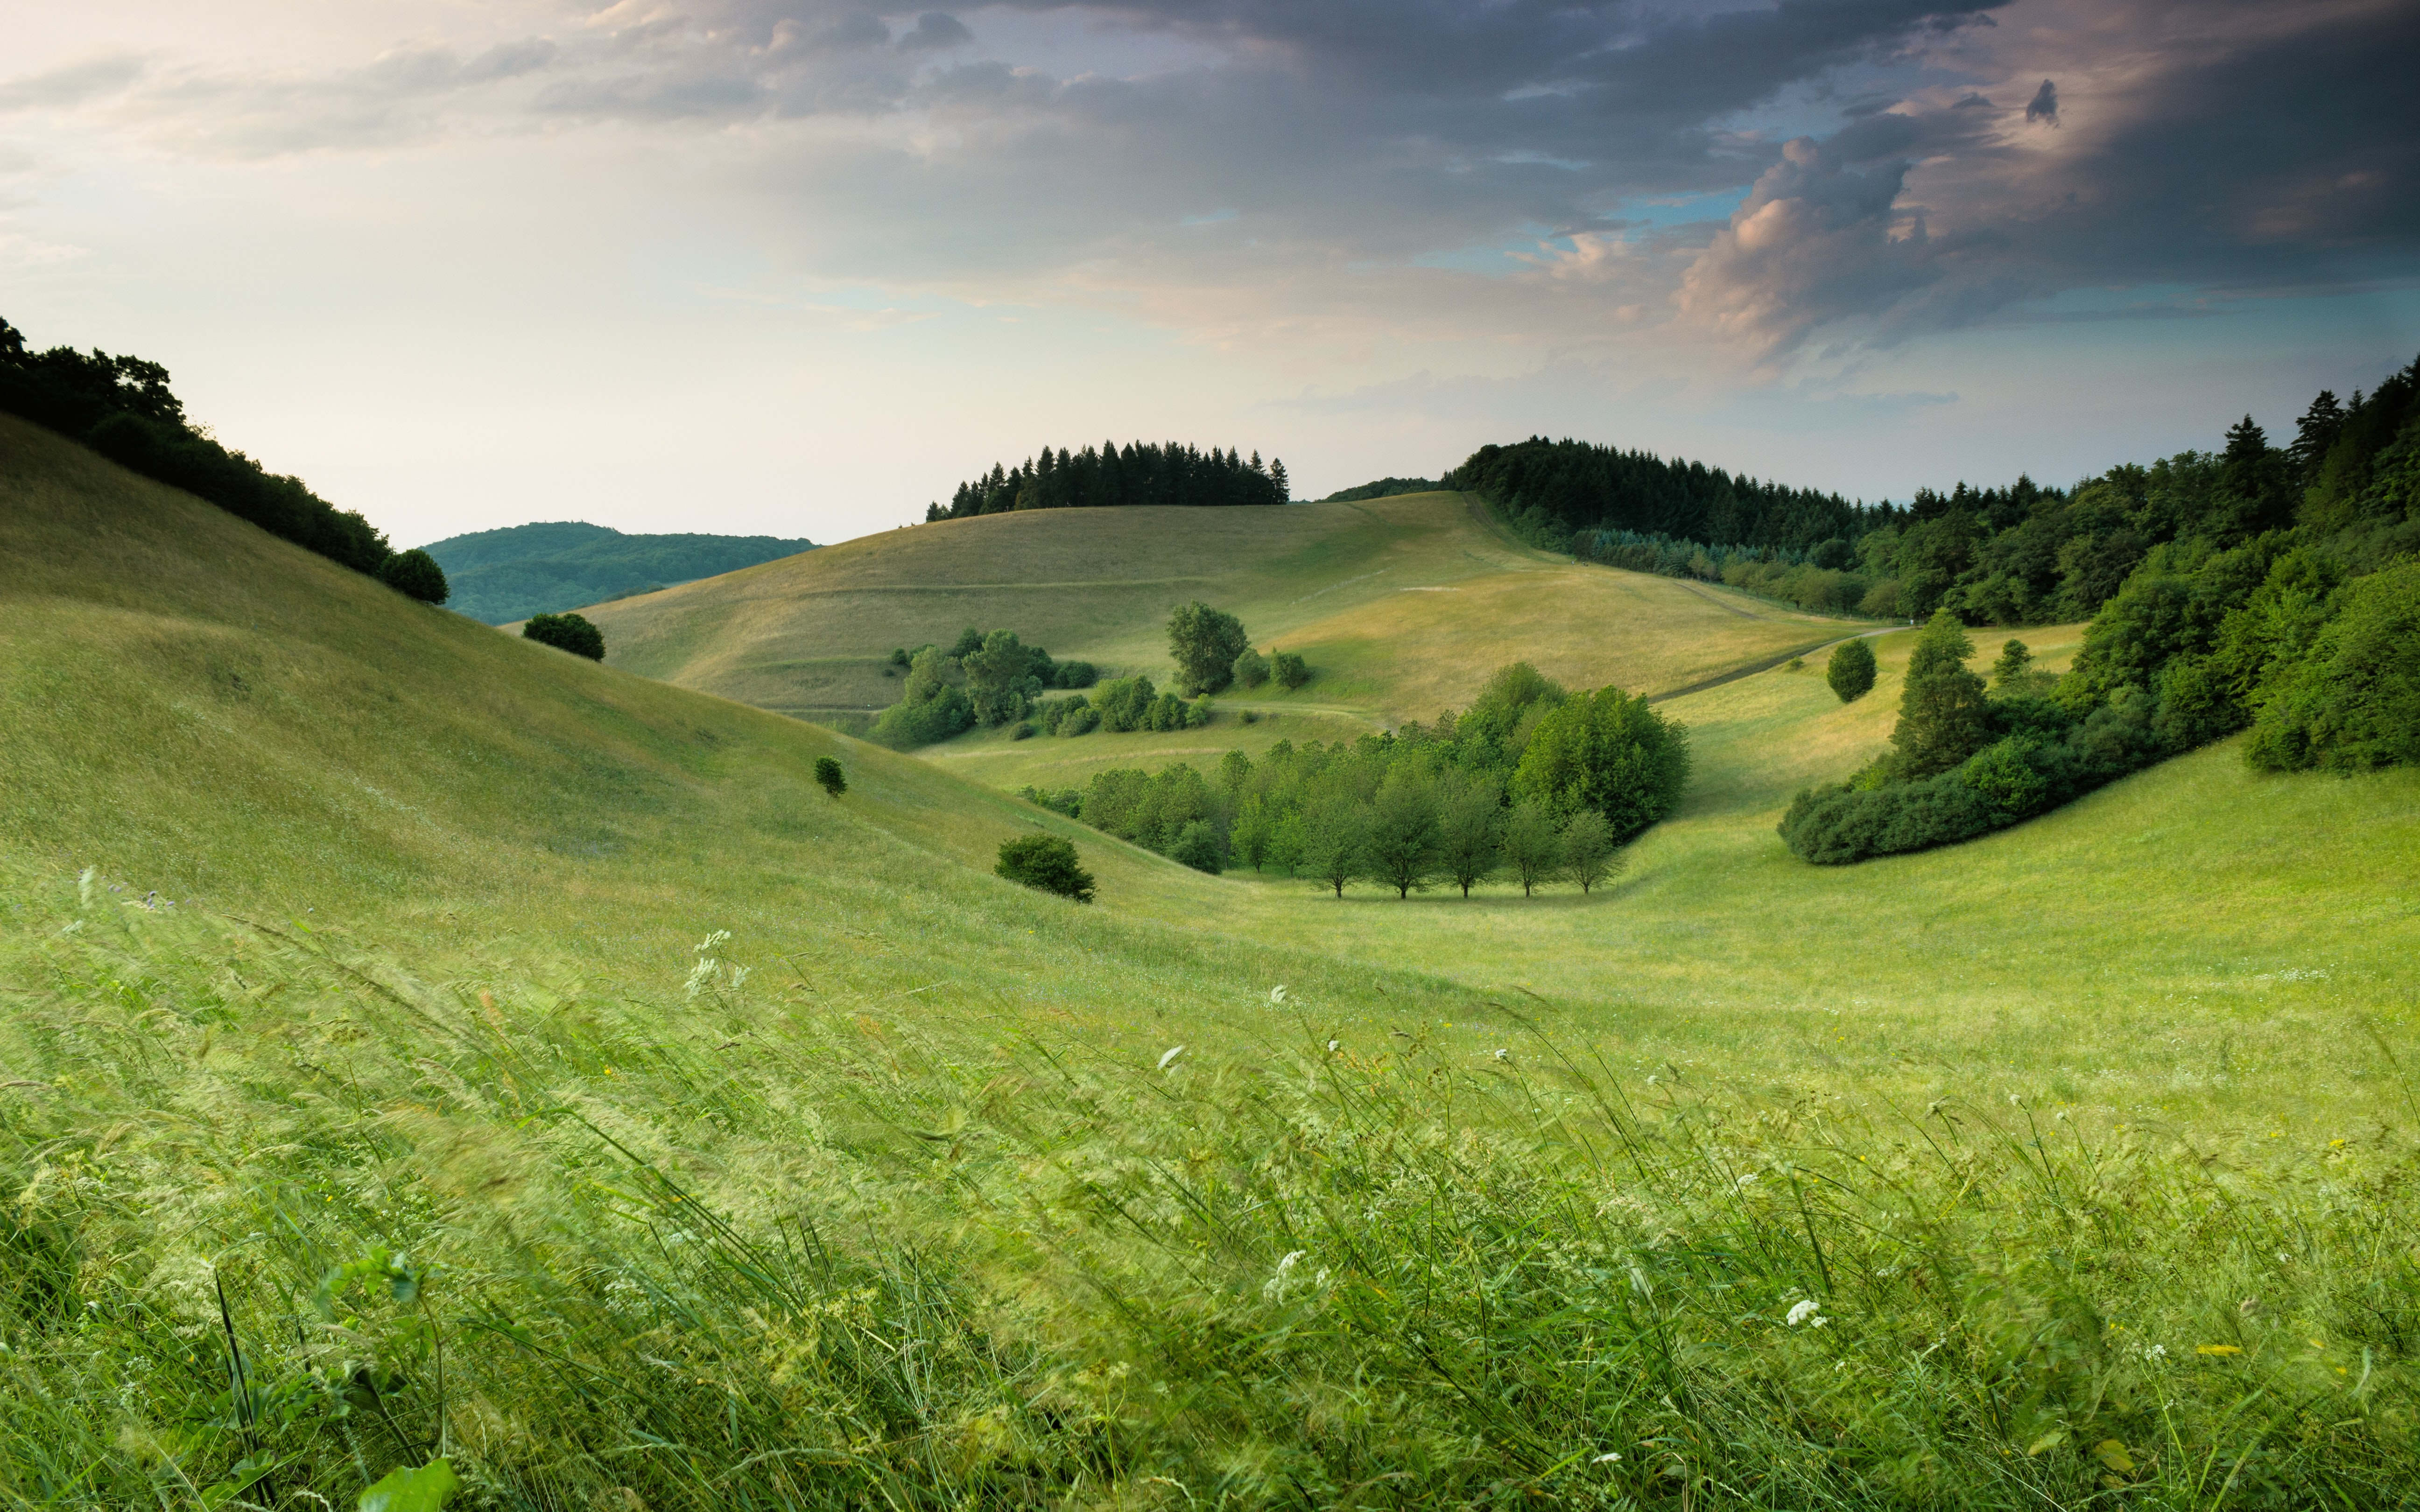
\includegraphics[width=\columnwidth]{./Figures/image2.jpg}
\captionof{figure}[Photo by Claudio Testa on Unsplash]{Photo by Claudio Testa on Unsplash} 
\label{fig:image2}
\end{minipage}

Proin maximus orci id ullamcorper blandit. Interdum et malesuada fames ac ante ipsum primis in faucibus. Mauris diam massa, sodales eu justo a, laoreet viverra quam. Vivamus vitae magna cursus, dignissim enim eget, ultrices turpis. Nunc faucibus faucibus dolor. Praesent congue fermentum viverra. Etiam venenatis ex ipsum. Phasellus semper tempus aliquet. Aenean id tellus condimentum, congue arcu id, bibendum odio. Praesent molestie elementum nulla. Proin ac condimentum sapien. Sed tempor orci sit amet mi luctus, eu tempus nisi pulvinar. Proin sit amet purus rutrum, accumsan ex varius, lacinia mauris. Sed sed fermentum neque. Maecenas eu vestibulum elit, ut imperdiet leo. Vestibulum tempor suscipit leo, eget interdum ligula malesuada a. Cras feugiat a nisl sit amet mattis. Vivamus varius commodo molestie \ref{fig:image2}.

Etiam elit mauris, mollis non nulla sit amet, porttitor dictum urna. Sed vitae volutpat nisl. Mauris egestas sollicitudin ante ut rutrum. Suspendisse non dui nec nulla tristique hendrerit quis ac eros. In porta ligula erat, blandit feugiat nulla pretium ac. In quis congue nisi, vulputate suscipit erat. Sed sit amet arcu vel ligula malesuada sollicitudin. Donec quis velit at nulla venenatis sodales ut a tellus. Phasellus semper vehicula mi, sed ultricies arcu tristique sit amet.


% full width figure
\begin{figure*}[ht!]
\begin{center}
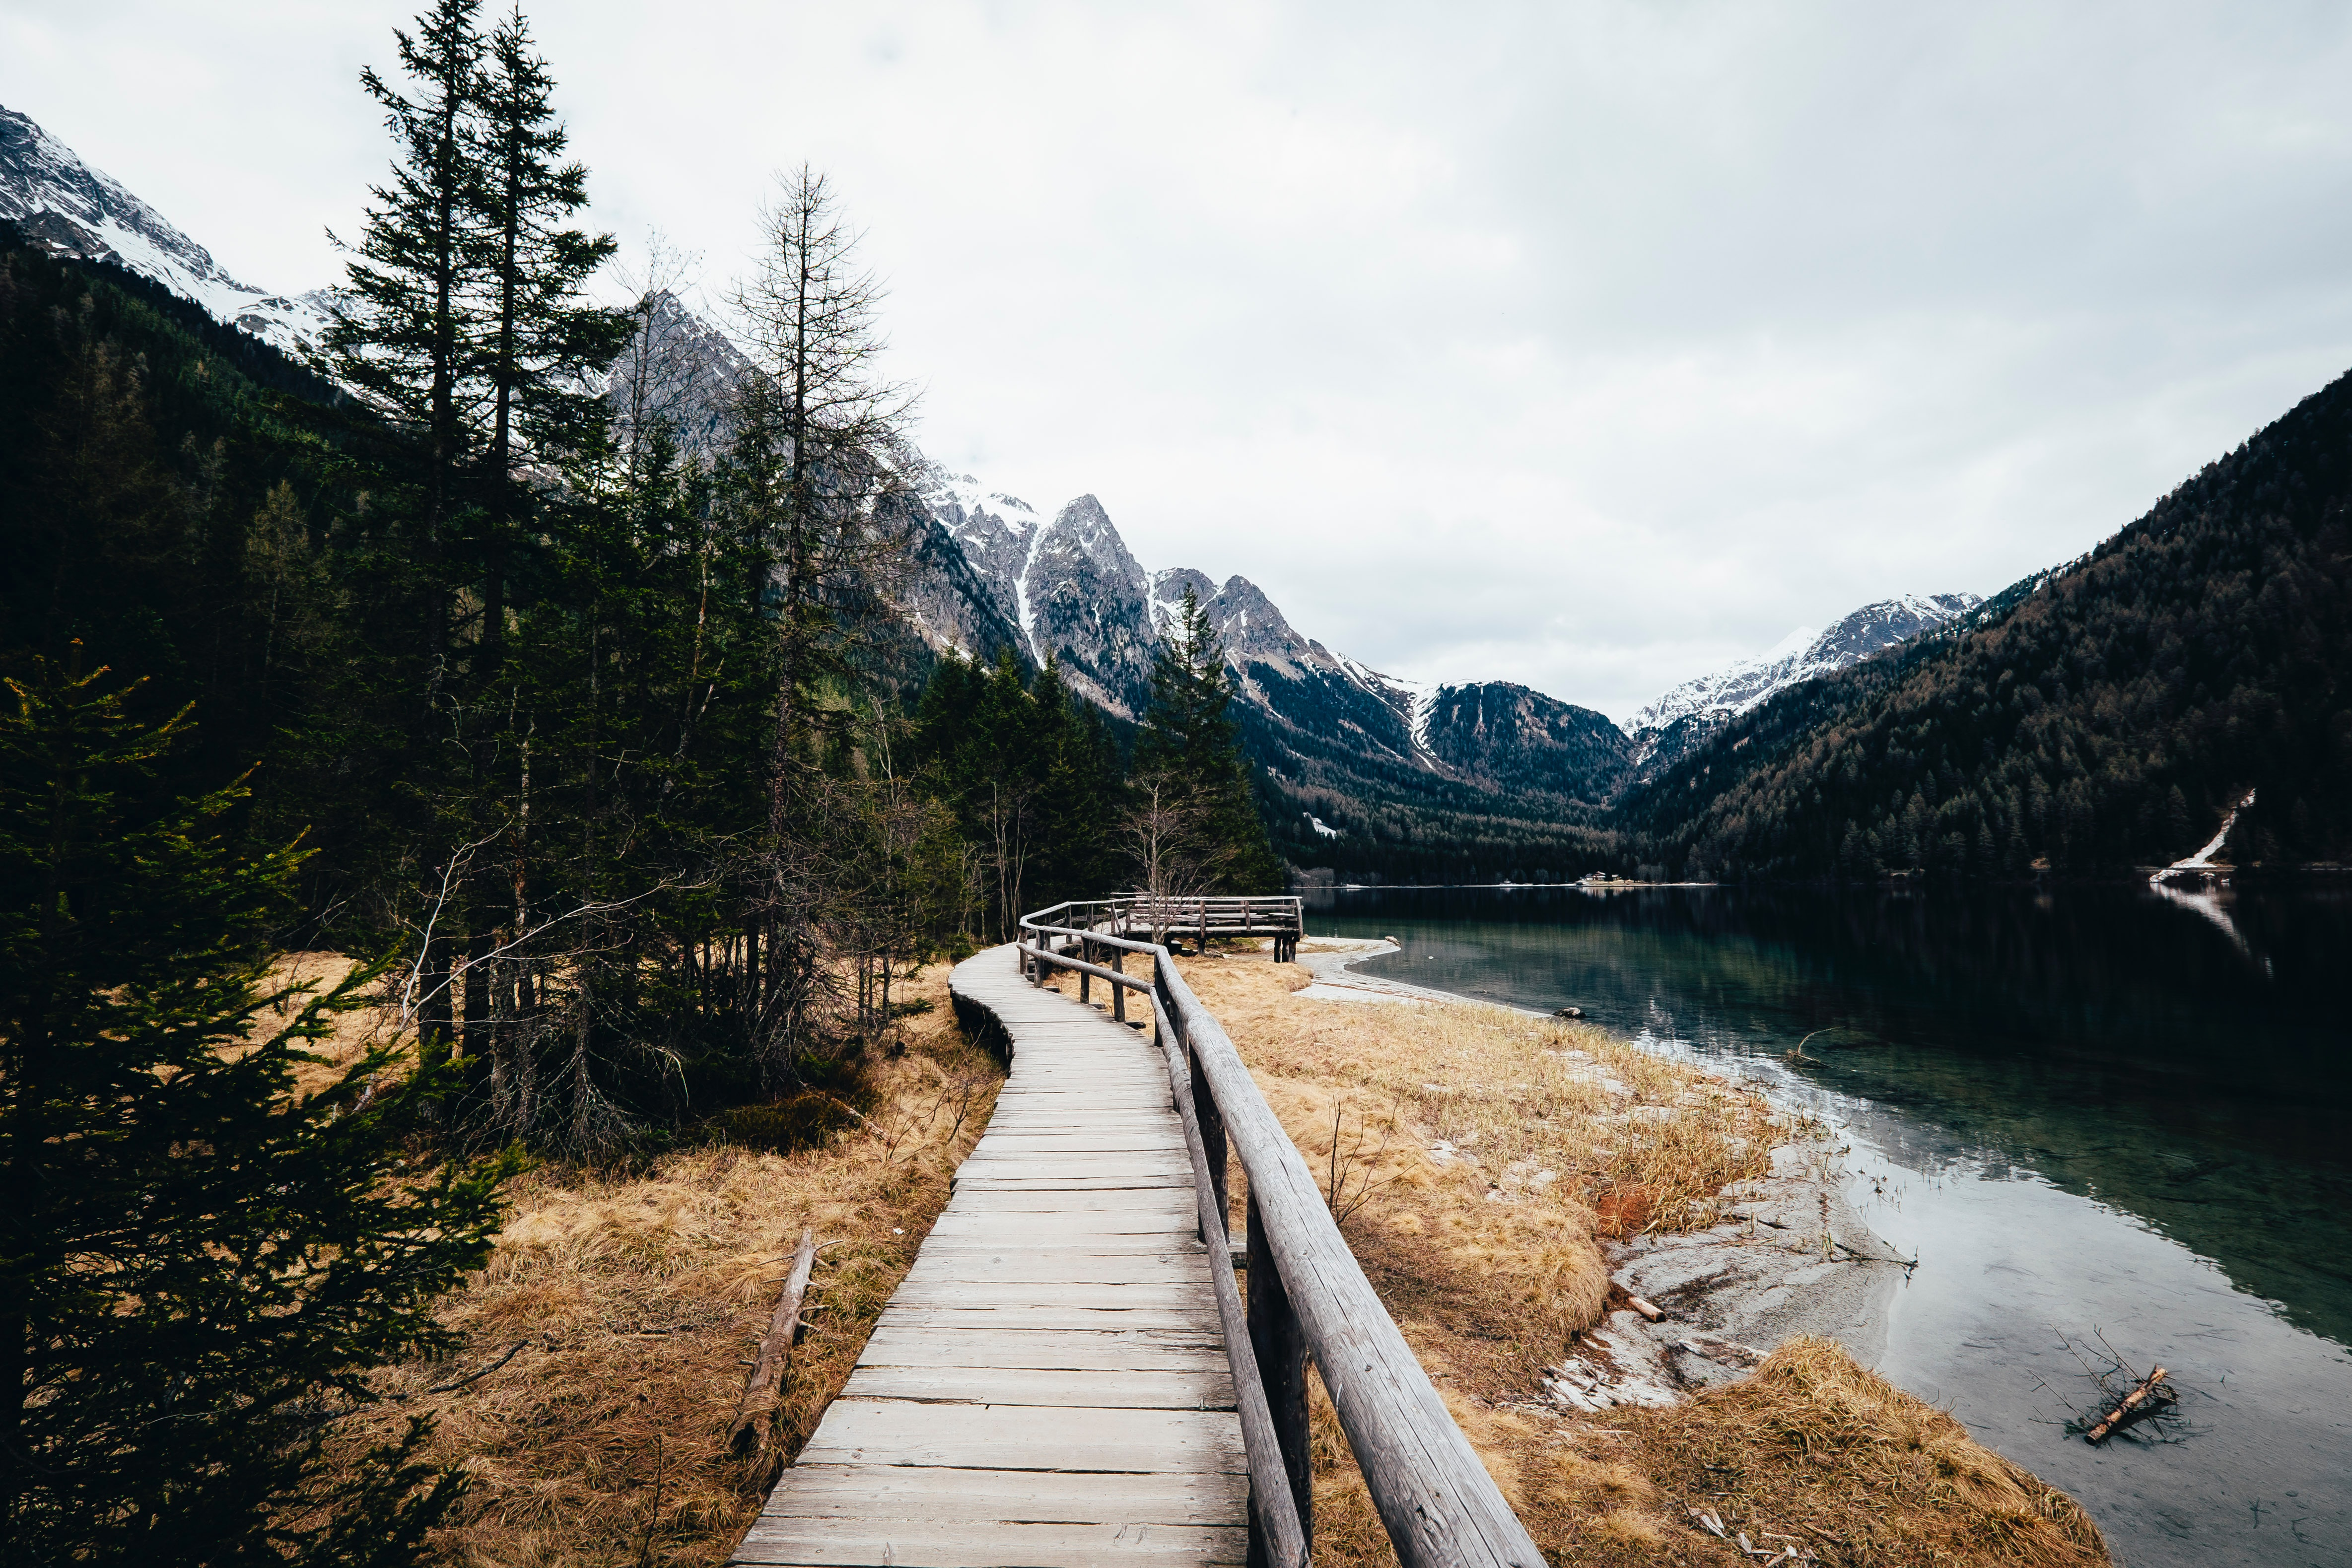
\includegraphics[width=0.9\linewidth]{./Figures/image1.jpg}
\captionof{figure}[Photo by Fabian Irsara on Unsplash]{Photo by Fabian Irsara on Unsplash}
\label{fig:image1}
\end{center}
\end{figure*}


Maecenas eget placerat dolor, id suscipit nisl. Aenean consectetur faucibus iaculis. Nulla rhoncus est ligula. Duis hendrerit molestie augue, sed vehicula nisl convallis eu. Phasellus ornare augue at quam finibus porttitor vel in nunc. Proin vitae tristique erat. Donec ullamcorper quam sollicitudin leo imperdiet, sed sollicitudin odio dictum. Mauris sed tellus et ligula consectetur maximus sit amet at sem. Cras neque orci, eleifend non laoreet vel, tristique eu ante. Fusce efficitur magna vitae magna eleifend eleifend. Quisque placerat vestibulum erat eget suscipit. Vestibulum vehicula tempor justo. Morbi interdum, felis in molestie vehicula, nunc erat mollis orci, ac placerat dolor leo nec ipsum. Ut ac ultricies ex. Quisque at metus mollis, tincidunt lorem vel, sollicitudin odio. Maecenas ut nibh ac ex malesuada maximus et vel nisi.

\section{Section}

\subsection{Subsection}
\label{subsec:subsectionname2}

Use section or subsection label for reference within text \ref{subsec:subsectionname2}.

\subsubsection{Sub sub subsection}

Many many layers of sections. Soooo many layers. I think they lose numbering at this level though.

For tables following the column width, see latex code below.

% column-width table
\noindent
\begin{minipage}[t]{0.45\textwidth}
\begin{center}
\label{tab:techspecs}
\captionof{table}{Caption of table. This is a column-width table.}
\begin{tabular}{l l}
\hline
                             & Subic Radar                                                                                                    \\ \hline
Polarization                 & Single-Pol                                                                                                     \\
Position (lat/lon)           & 14.82$^{\circ} N$ 120.36 $^{\circ} E$                                                                            \\
Altitude 		             & 532 m.a.s.l.                                                                                                           \\
Maximum Range                & 120 km (150 km)                                                                                                         \\
Azimuth resolution           & 1 $^{\circ}$                                                                                                    \\
Beam width                   & 0.95 $^{\circ}$                                                                                                    \\
Gate length                  & 500 m (250 m)                                                                                                          \\
Number of elevation angles   & 14 (3)                                                                                                            \\
\hline
%Elevation angles             & \begin{tabular}[c]{@{}l@{}}0.5, 1.5, 2.4, 3.4, 4.3, 5.3, 6.2, 7.5, 8.7, 10, 12, 14, 16.7, 19.5 ($^{\circ}$) \\(0.0, 1.0, 2.0)\end{tabular} \\
Elevation angles             & 0.5, 1.5, 2.4, 3.4, 4.3, \\
& 5.3, 6.2, 7.5, 8.7, 10, \\ & 12, 14, 16.7, 19.5 ($^{\circ}$) \\ 
&(0.0, 1.0, 2.0)
\\
\hline
Volume cycle interval        & 9 minutes                                                                                                      \\
Data available since         & April 2012                                                                                                     \\
Peak power                   & 850 kW                                                                                                         \\
Wavelength                   & 10.7 cm                                                                                                        \\ \hline
\end{tabular}
\end{center}
\end{minipage}%


Proin maximus orci id ullamcorper blandit. Interdum et malesuada fames ac ante ipsum primis in faucibus. Mauris diam massa, sodales eu justo a, laoreet viverra quam. Vivamus vitae magna cursus, dignissim enim eget, ultrices turpis. Nunc faucibus faucibus dolor. Praesent congue fermentum viverra. Etiam venenatis ex ipsum.

% Full width table
\begin{table*}
\begin{center}
\caption{Caption of table. This is a full-width table.}
\begin{tabular}{@{}lcc@{}}
\toprule
                           & \multicolumn{1}{c}{Subic Radar}                  & \multicolumn{1}{c}{Tagaytay Radar}                 \\ \midrule
Bandwidth                  & S-Band                                           & C-Band                                             \\
Polarization               & Single-pol                                       & Dual-pol                                           \\
Position (lat/lon)         & 14.822°N 120.363°E                               & 14.123°N 120.974°E                                 \\
Altitude                   & 532 m a.s.l.                                     & 752 m a.s.l.                                       \\
Maximum Range              & \multicolumn{2}{c}{120 km}                                                                            \\
Azimuth Resolution         & \multicolumn{2}{c}{1 $^{\circ}$}                                                                      \\
Gate length                & \multicolumn{2}{c}{500 m}                                                                             \\
Number of elevation angles & \multicolumn{2}{c}{14}                                                                                \\
Elevation angles           & \multicolumn{2}{c}{0.5°, 1.5°, 2.4°, 3.4°, 4.3°, 5.3°, 6.2°, 7.5°, 8.7°, 10°, 12°, 14°, 16.7°, 19.5°} \\
Volume cycle interval      & 8 minutes                                        & 15 minutes                                         \\
Start of operation         & 2012                                             & 2012                                               \\ \bottomrule
\end{tabular}
\label{tab:SUBtechspecs}
\end{center}
\end{table*}%


\end{multicols}

\newpage

\section*{Supplemental material to the manuscript}

% going back to single column

Nullam et semper lectus, sit amet condimentum lorem. Quisque tempus felis massa, ac molestie tellus pharetra non. Nam mollis vel urna in malesuada. Duis ultricies congue enim vitae lobortis. Maecenas consequat mi ac ligula consequat gravida. Pellentesque sed mauris iaculis, posuere dui non, porttitor turpis. Suspendisse ornare urna felis, eget luctus enim posuere quis. Pellentesque non auctor ligula. Suspendisse porta orci id ultrices facilisis.
